\documentclass[11pt,compress,t,notes=noshow, xcolor=table]{beamer}
\usepackage[]{graphicx}\usepackage[]{color}
% maxwidth is the original width if it is less than linewidth
% otherwise use linewidth (to make sure the graphics do not exceed the margin)
\makeatletter
\def\maxwidth{ %
  \ifdim\Gin@nat@width>\linewidth
    \linewidth
  \else
    \Gin@nat@width
  \fi
}
\makeatother

\definecolor{fgcolor}{rgb}{0.345, 0.345, 0.345}
\newcommand{\hlnum}[1]{\textcolor[rgb]{0.686,0.059,0.569}{#1}}%
\newcommand{\hlstr}[1]{\textcolor[rgb]{0.192,0.494,0.8}{#1}}%
\newcommand{\hlcom}[1]{\textcolor[rgb]{0.678,0.584,0.686}{\textit{#1}}}%
\newcommand{\hlopt}[1]{\textcolor[rgb]{0,0,0}{#1}}%
\newcommand{\hlstd}[1]{\textcolor[rgb]{0.345,0.345,0.345}{#1}}%
\newcommand{\hlkwa}[1]{\textcolor[rgb]{0.161,0.373,0.58}{\textbf{#1}}}%
\newcommand{\hlkwb}[1]{\textcolor[rgb]{0.69,0.353,0.396}{#1}}%
\newcommand{\hlkwc}[1]{\textcolor[rgb]{0.333,0.667,0.333}{#1}}%
\newcommand{\hlkwd}[1]{\textcolor[rgb]{0.737,0.353,0.396}{\textbf{#1}}}%
\let\hlipl\hlkwb

\usepackage{framed}
\makeatletter
\newenvironment{kframe}{%
 \def\at@end@of@kframe{}%
 \ifinner\ifhmode%
  \def\at@end@of@kframe{\end{minipage}}%
  \begin{minipage}{\columnwidth}%
 \fi\fi%
 \def\FrameCommand##1{\hskip\@totalleftmargin \hskip-\fboxsep
 \colorbox{shadecolor}{##1}\hskip-\fboxsep
     % There is no \\@totalrightmargin, so:
     \hskip-\linewidth \hskip-\@totalleftmargin \hskip\columnwidth}%
 \MakeFramed {\advance\hsize-\width
   \@totalleftmargin\z@ \linewidth\hsize
   \@setminipage}}%
 {\par\unskip\endMakeFramed%
 \at@end@of@kframe}
\makeatother

\definecolor{shadecolor}{rgb}{.97, .97, .97}
\definecolor{messagecolor}{rgb}{0, 0, 0}
\definecolor{warningcolor}{rgb}{1, 0, 1}
\definecolor{errorcolor}{rgb}{1, 0, 0}
\newenvironment{knitrout}{}{} % an empty environment to be redefined in TeX

\usepackage{alltt}
\newcommand{\SweaveOpts}[1]{}  % do not interfere with LaTeX
\newcommand{\SweaveInput}[1]{} % because they are not real TeX commands
\newcommand{\Sexpr}[1]{}       % will only be parsed by R
\newcommand{\xmark}{\ding{55}}%


\usepackage[english]{babel}
\usepackage[utf8]{inputenc}

\usepackage{dsfont}
\usepackage{verbatim}
\usepackage{amsmath}
\usepackage{amsfonts}
\usepackage{amssymb}
\usepackage{bm}
\usepackage{csquotes}
\usepackage{multirow}
\usepackage{longtable}
\usepackage{booktabs}
\usepackage{enumerate}
\usepackage[absolute,overlay]{textpos}
\usepackage{psfrag}
\usepackage{algorithm}
\usepackage{algpseudocode}
\usepackage{eqnarray}
\usepackage{arydshln}
\usepackage{tabularx}
\usepackage{placeins}
\usepackage{tikz}
\usepackage{setspace}
\usepackage{colortbl}
\usepackage{mathtools}
\usepackage{wrapfig}
\usepackage{bm}
\usepackage{amsmath}
\usepackage{pifont}

\usetikzlibrary{shapes,arrows,automata,positioning,calc,chains,trees, shadows}
\tikzset{
  %Define standard arrow tip
  >=stealth',
  %Define style for boxes
  punkt/.style={
    rectangle,
    rounded corners,
    draw=black, very thick,
    text width=6.5em,
    minimum height=2em,
    text centered},
  % Define arrow style
  pil/.style={
    ->,
    thick,
    shorten <=2pt,
    shorten >=2pt,}
}

\usepackage{subfig}

% Defines macros and environments
\usepackage{../../style/lmu-lecture}


\let\code=\texttt
\let\proglang=\textsf

\setkeys{Gin}{width=0.9\textwidth}

\setbeamertemplate{frametitle}{\expandafter\uppercase\expandafter\insertframetitle}

\usepackage{bbm}
% basic latex stuff
\newcommand{\pkg}[1]{{\fontseries{b}\selectfont #1}} %fontstyle for R packages
\newcommand{\lz}{\vspace{0.5cm}} %vertical space
\newcommand{\dlz}{\vspace{1cm}} %double vertical space
\newcommand{\oneliner}[1] % Oneliner for important statements
{\begin{block}{}\begin{center}\begin{Large}#1\end{Large}\end{center}\end{block}}


%new environments
\newenvironment{vbframe}  %frame with breaks and verbatim
{
 \begin{frame}[containsverbatim,allowframebreaks]
}
{
\end{frame}
}

\newenvironment{vframe}  %frame with verbatim without breaks (to avoid numbering one slided frames)
{
 \begin{frame}[containsverbatim]
}
{
\end{frame}
}

\newenvironment{blocki}[1]   % itemize block
{
 \begin{block}{#1}\begin{itemize}
}
{
\end{itemize}\end{block}
}

\newenvironment{fragileframe}[2]{  %fragile frame with framebreaks
\begin{frame}[allowframebreaks, fragile, environment = fragileframe]
\frametitle{#1}
#2}
{\end{frame}}


\newcommand{\myframe}[2]{  %short for frame with framebreaks
\begin{frame}[allowframebreaks]
\frametitle{#1}
#2
\end{frame}}

\newcommand{\remark}[1]{
  \textbf{Remark:} #1
}

\newcommand{\citebutton}[2]{%
\NoCaseChange{\resizebox{!}{9pt}{\protect\beamergotobutton{\href{#2}{#1}}}}%
}



\newenvironment{deleteframe}
{
\begingroup
\usebackgroundtemplate{\includegraphics[width=\paperwidth,height=\paperheight]{../style/color/red.png}}
 \begin{frame}
}
{
\end{frame}
\endgroup
}
\newenvironment{simplifyframe}
{
\begingroup
\usebackgroundtemplate{\includegraphics[width=\paperwidth,height=\paperheight]{../style/color/yellow.png}}
 \begin{frame}
}
{
\end{frame}
\endgroup
}\newenvironment{draftframe}
{
\begingroup
\usebackgroundtemplate{\includegraphics[width=\paperwidth,height=\paperheight]{../style/color/green.jpg}}
 \begin{frame}
}
{
\end{frame}
\endgroup
}
% https://tex.stackexchange.com/a/261480: textcolor that works in mathmode
\makeatletter
\renewcommand*{\@textcolor}[3]{%
  \protect\leavevmode
  \begingroup
    \color#1{#2}#3%
  \endgroup
}
\makeatother





% math spaces
\ifdefined\N                                                                
\renewcommand{\N}{\mathds{N}} % N, naturals
\else \newcommand{\N}{\mathds{N}} \fi 
\newcommand{\Z}{\mathds{Z}} % Z, integers
\newcommand{\Q}{\mathds{Q}} % Q, rationals
\newcommand{\R}{\mathds{R}} % R, reals
\ifdefined\C 
  \renewcommand{\C}{\mathds{C}} % C, complex
\else \newcommand{\C}{\mathds{C}} \fi
\newcommand{\continuous}{\mathcal{C}} % C, space of continuous functions
\newcommand{\M}{\mathcal{M}} % machine numbers
\newcommand{\epsm}{\epsilon_m} % maximum error

% counting / finite sets
\newcommand{\setzo}{\{0, 1\}} % set 0, 1
\newcommand{\setmp}{\{-1, +1\}} % set -1, 1
\newcommand{\unitint}{[0, 1]} % unit interval

% basic math stuff
\newcommand{\xt}{\tilde x} % x tilde
\newcommand{\argmax}{\operatorname{arg\,max}} % argmax
\newcommand{\argmin}{\operatorname{arg\,min}} % argmin
\newcommand{\argminlim}{\mathop{\mathrm{arg\,min}}\limits} % argmax with limits
\newcommand{\argmaxlim}{\mathop{\mathrm{arg\,max}}\limits} % argmin with limits  
\newcommand{\sign}{\operatorname{sign}} % sign, signum
\newcommand{\I}{\mathbb{I}} % I, indicator
\newcommand{\order}{\mathcal{O}} % O, order
\newcommand{\pd}[2]{\frac{\partial{#1}}{\partial #2}} % partial derivative
\newcommand{\floorlr}[1]{\left\lfloor #1 \right\rfloor} % floor
\newcommand{\ceillr}[1]{\left\lceil #1 \right\rceil} % ceiling

% sums and products
\newcommand{\sumin}{\sum\limits_{i=1}^n} % summation from i=1 to n
\newcommand{\sumim}{\sum\limits_{i=1}^m} % summation from i=1 to m
\newcommand{\sumjn}{\sum\limits_{j=1}^n} % summation from j=1 to p
\newcommand{\sumjp}{\sum\limits_{j=1}^p} % summation from j=1 to p
\newcommand{\sumik}{\sum\limits_{i=1}^k} % summation from i=1 to k
\newcommand{\sumkg}{\sum\limits_{k=1}^g} % summation from k=1 to g
\newcommand{\sumjg}{\sum\limits_{j=1}^g} % summation from j=1 to g
\newcommand{\meanin}{\frac{1}{n} \sum\limits_{i=1}^n} % mean from i=1 to n
\newcommand{\meanim}{\frac{1}{m} \sum\limits_{i=1}^m} % mean from i=1 to n
\newcommand{\meankg}{\frac{1}{g} \sum\limits_{k=1}^g} % mean from k=1 to g
\newcommand{\prodin}{\prod\limits_{i=1}^n} % product from i=1 to n
\newcommand{\prodkg}{\prod\limits_{k=1}^g} % product from k=1 to g
\newcommand{\prodjp}{\prod\limits_{j=1}^p} % product from j=1 to p

% linear algebra
\newcommand{\one}{\boldsymbol{1}} % 1, unitvector
\newcommand{\zero}{\mathbf{0}} % 0-vector
\newcommand{\id}{\boldsymbol{I}} % I, identity
\newcommand{\diag}{\operatorname{diag}} % diag, diagonal
\newcommand{\trace}{\operatorname{tr}} % tr, trace
\newcommand{\spn}{\operatorname{span}} % span
\newcommand{\scp}[2]{\left\langle #1, #2 \right\rangle} % <.,.>, scalarproduct
\newcommand{\mat}[1]{\begin{pmatrix} #1 \end{pmatrix}} % short pmatrix command
\newcommand{\Amat}{\mathbf{A}} % matrix A
\newcommand{\Deltab}{\mathbf{\Delta}} % error term for vectors

% basic probability + stats
\renewcommand{\P}{\mathds{P}} % P, probability
\newcommand{\E}{\mathds{E}} % E, expectation
\newcommand{\var}{\mathsf{Var}} % Var, variance
\newcommand{\cov}{\mathsf{Cov}} % Cov, covariance
\newcommand{\corr}{\mathsf{Corr}} % Corr, correlation
\newcommand{\normal}{\mathcal{N}} % N of the normal distribution
\newcommand{\iid}{\overset{i.i.d}{\sim}} % dist with i.i.d superscript
\newcommand{\distas}[1]{\overset{#1}{\sim}} % ... is distributed as ...

% machine learning
\newcommand{\Xspace}{\mathcal{X}} % X, input space
\newcommand{\Yspace}{\mathcal{Y}} % Y, output space
\newcommand{\nset}{\{1, \ldots, n\}} % set from 1 to n
\newcommand{\pset}{\{1, \ldots, p\}} % set from 1 to p
\newcommand{\gset}{\{1, \ldots, g\}} % set from 1 to g
\newcommand{\Pxy}{\mathbb{P}_{xy}} % P_xy
\newcommand{\Exy}{\mathbb{E}_{xy}} % E_xy: Expectation over random variables xy
\newcommand{\xv}{\mathbf{x}} % vector x (bold)
\newcommand{\xtil}{\tilde{\mathbf{x}}} % vector x-tilde (bold)
\newcommand{\yv}{\mathbf{y}} % vector y (bold)
\newcommand{\xy}{(\xv, y)} % observation (x, y)
\newcommand{\xvec}{\left(x_1, \ldots, x_p\right)^\top} % (x1, ..., xp) 
\newcommand{\Xmat}{\mathbf{X}} % Design matrix
\newcommand{\allDatasets}{\mathds{D}} % The set of all datasets
\newcommand{\allDatasetsn}{\mathds{D}_n}  % The set of all datasets of size n 
\newcommand{\D}{\mathcal{D}} % D, data
\newcommand{\Dn}{\D_n} % D_n, data of size n
\newcommand{\Dtrain}{\mathcal{D}_{\text{train}}} % D_train, training set
\newcommand{\Dtest}{\mathcal{D}_{\text{test}}} % D_test, test set
\newcommand{\xyi}[1][i]{\left(\xv^{(#1)}, y^{(#1)}\right)} % (x^i, y^i), i-th observation
\newcommand{\Dset}{\left( \xyi[1], \ldots, \xyi[n]\right)} % {(x1,y1)), ..., (xn,yn)}, data
\newcommand{\defAllDatasetsn}{(\Xspace \times \Yspace)^n} % Def. of the set of all datasets of size n 
\newcommand{\defAllDatasets}{\bigcup_{n \in \N}(\Xspace \times \Yspace)^n} % Def. of the set of all datasets 
\newcommand{\xdat}{\left\{ \xv^{(1)}, \ldots, \xv^{(n)}\right\}} % {x1, ..., xn}, input data
\newcommand{\yvec}{\left(y^{(1)}, \hdots, y^{(n)}\right)^\top} % (y1, ..., yn), vector of outcomes
\renewcommand{\xi}[1][i]{\xv^{(#1)}} % x^i, i-th observed value of x
\newcommand{\yi}[1][i]{y^{(#1)}} % y^i, i-th observed value of y 
\newcommand{\xivec}{\left(x^{(i)}_1, \ldots, x^{(i)}_p\right)^\top} % (x1^i, ..., xp^i), i-th observation vector
\newcommand{\xj}{\xv_j} % x_j, j-th feature
\newcommand{\xjvec}{\left(x^{(1)}_j, \ldots, x^{(n)}_j\right)^\top} % (x^1_j, ..., x^n_j), j-th feature vector
\newcommand{\phiv}{\mathbf{\phi}} % Basis transformation function phi
\newcommand{\phixi}{\mathbf{\phi}^{(i)}} % Basis transformation of xi: phi^i := phi(xi)

%%%%%% ml - models general
\newcommand{\lamv}{\bm{\lambda}} % lambda vector, hyperconfiguration vector
\newcommand{\Lam}{\bm{\Lambda}}	 % Lambda, space of all hpos
% Inducer / Inducing algorithm
\newcommand{\preimageInducer}{\left(\defAllDatasets\right)\times\Lam} % Set of all datasets times the hyperparameter space
\newcommand{\preimageInducerShort}{\allDatasets\times\Lam} % Set of all datasets times the hyperparameter space
% Inducer / Inducing algorithm
\newcommand{\ind}{\mathcal{I}} % Inducer, inducing algorithm, learning algorithm 

% continuous prediction function f
\newcommand{\ftrue}{f_{\text{true}}}  % True underlying function (if a statistical model is assumed)
\newcommand{\ftruex}{\ftrue(\xv)} % True underlying function (if a statistical model is assumed)
\newcommand{\fx}{f(\xv)} % f(x), continuous prediction function
\newcommand{\fdomains}{f: \Xspace \rightarrow \R^g} % f with domain and co-domain
\newcommand{\Hspace}{\mathcal{H}} % hypothesis space where f is from
\newcommand{\fbayes}{f^{\ast}} % Bayes-optimal model
\newcommand{\fxbayes}{f^{\ast}(\xv)} % Bayes-optimal model
\newcommand{\fkx}[1][k]{f_{#1}(\xv)} % f_j(x), discriminant component function
\newcommand{\fh}{\hat{f}} % f hat, estimated prediction function
\newcommand{\fxh}{\fh(\xv)} % fhat(x)
\newcommand{\fxt}{f(\xv ~|~ \thetab)} % f(x | theta)
\newcommand{\fxi}{f\left(\xv^{(i)}\right)} % f(x^(i))
\newcommand{\fxih}{\hat{f}\left(\xv^{(i)}\right)} % f(x^(i))
\newcommand{\fxit}{f\left(\xv^{(i)} ~|~ \thetab\right)} % f(x^(i) | theta)
\newcommand{\fhD}{\fh_{\D}} % fhat_D, estimate of f based on D
\newcommand{\fhDtrain}{\fh_{\Dtrain}} % fhat_Dtrain, estimate of f based on D
\newcommand{\fhDnlam}{\fh_{\Dn, \lamv}} %model learned on Dn with hp lambda
\newcommand{\fhDlam}{\fh_{\D, \lamv}} %model learned on D with hp lambda
\newcommand{\fhDnlams}{\fh_{\Dn, \lamv^\ast}} %model learned on Dn with optimal hp lambda 
\newcommand{\fhDlams}{\fh_{\D, \lamv^\ast}} %model learned on D with optimal hp lambda 

% discrete prediction function h
\newcommand{\hx}{h(\xv)} % h(x), discrete prediction function
\newcommand{\hh}{\hat{h}} % h hat
\newcommand{\hxh}{\hat{h}(\xv)} % hhat(x)
\newcommand{\hxt}{h(\xv | \thetab)} % h(x | theta)
\newcommand{\hxi}{h\left(\xi\right)} % h(x^(i))
\newcommand{\hxit}{h\left(\xi ~|~ \thetab\right)} % h(x^(i) | theta)
\newcommand{\hbayes}{h^{\ast}} % Bayes-optimal classification model
\newcommand{\hxbayes}{h^{\ast}(\xv)} % Bayes-optimal classification model

% yhat
\newcommand{\yh}{\hat{y}} % yhat for prediction of target
\newcommand{\yih}{\hat{y}^{(i)}} % yhat^(i) for prediction of ith targiet
\newcommand{\resi}{\yi- \yih}

% theta
\newcommand{\thetah}{\hat{\theta}} % theta hat
\newcommand{\thetab}{\bm{\theta}} % theta vector
\newcommand{\thetabh}{\bm{\hat\theta}} % theta vector hat
\newcommand{\thetat}[1][t]{\thetab^{[#1]}} % theta^[t] in optimization
\newcommand{\thetatn}[1][t]{\thetab^{[#1 +1]}} % theta^[t+1] in optimization
\newcommand{\thetahDnlam}{\thetabh_{\Dn, \lamv}} %theta learned on Dn with hp lambda
\newcommand{\thetahDlam}{\thetabh_{\D, \lamv}} %theta learned on D with hp lambda
\newcommand{\mint}{\min_{\thetab \in \Theta}} % min problem theta
\newcommand{\argmint}{\argmin_{\thetab \in \Theta}} % argmin theta

% densities + probabilities
% pdf of x 
\newcommand{\pdf}{p} % p
\newcommand{\pdfx}{p(\xv)} % p(x)
\newcommand{\pixt}{\pi(\xv~|~ \thetab)} % pi(x|theta), pdf of x given theta
\newcommand{\pixit}{\pi\left(\xi ~|~ \thetab\right)} % pi(x^i|theta), pdf of x given theta
\newcommand{\pixii}{\pi\left(\xi\right)} % pi(x^i), pdf of i-th x 

% pdf of (x, y)
\newcommand{\pdfxy}{p(\xv,y)} % p(x, y)
\newcommand{\pdfxyt}{p(\xv, y ~|~ \thetab)} % p(x, y | theta)
\newcommand{\pdfxyit}{p\left(\xi, \yi ~|~ \thetab\right)} % p(x^(i), y^(i) | theta)

% pdf of x given y
\newcommand{\pdfxyk}[1][k]{p(\xv | y= #1)} % p(x | y = k)
\newcommand{\lpdfxyk}[1][k]{\log p(\xv | y= #1)} % log p(x | y = k)
\newcommand{\pdfxiyk}[1][k]{p\left(\xi | y= #1 \right)} % p(x^i | y = k)

% prior probabilities
\newcommand{\pik}[1][k]{\pi_{#1}} % pi_k, prior
\newcommand{\lpik}[1][k]{\log \pi_{#1}} % log pi_k, log of the prior
\newcommand{\pit}{\pi(\thetab)} % Prior probability of parameter theta

% posterior probabilities
\newcommand{\post}{\P(y = 1 ~|~ \xv)} % P(y = 1 | x), post. prob for y=1
\newcommand{\postk}[1][k]{\P(y = #1 ~|~ \xv)} % P(y = k | y), post. prob for y=k
\newcommand{\pidomains}{\pi: \Xspace \rightarrow \unitint} % pi with domain and co-domain
\newcommand{\pibayes}{\pi^{\ast}} % Bayes-optimal classification model
\newcommand{\pixbayes}{\pi^{\ast}(\xv)} % Bayes-optimal classification model
\newcommand{\pix}{\pi(\xv)} % pi(x), P(y = 1 | x)
\newcommand{\pikx}[1][k]{\pi_{#1}(\xv)} % pi_k(x), P(y = k | x)
\newcommand{\pikxt}[1][k]{\pi_{#1}(\xv ~|~ \thetab)} % pi_k(x | theta), P(y = k | x, theta)
\newcommand{\pixh}{\hat \pi(\xv)} % pi(x) hat, P(y = 1 | x) hat
\newcommand{\pikxh}[1][k]{\hat \pi_{#1}(\xv)} % pi_k(x) hat, P(y = k | x) hat
\newcommand{\pixih}{\hat \pi(\xi)} % pi(x^(i)) with hat
\newcommand{\pikxih}[1][k]{\hat \pi_{#1}(\xi)} % pi_k(x^(i)) with hat
\newcommand{\pdfygxt}{p(y ~|~\xv, \thetab)} % p(y | x, theta)
\newcommand{\pdfyigxit}{p\left(\yi ~|~\xi, \thetab\right)} % p(y^i |x^i, theta)
\newcommand{\lpdfygxt}{\log \pdfygxt } % log p(y | x, theta)
\newcommand{\lpdfyigxit}{\log \pdfyigxit} % log p(y^i |x^i, theta)

% probababilistic
\newcommand{\bayesrulek}[1][k]{\frac{\P(\xv | y= #1) \P(y= #1)}{\P(\xv)}} % Bayes rule
\newcommand{\muk}{\bm{\mu_k}} % mean vector of class-k Gaussian (discr analysis) 

% residual and margin
\newcommand{\eps}{\epsilon} % residual, stochastic
\newcommand{\epsi}{\epsilon^{(i)}} % epsilon^i, residual, stochastic
\newcommand{\epsh}{\hat{\epsilon}} % residual, estimated
\newcommand{\yf}{y \fx} % y f(x), margin
\newcommand{\yfi}{\yi \fxi} % y^i f(x^i), margin
\newcommand{\Sigmah}{\hat \Sigma} % estimated covariance matrix
\newcommand{\Sigmahj}{\hat \Sigma_j} % estimated covariance matrix for the j-th class

% ml - loss, risk, likelihood
\newcommand{\Lyf}{L\left(y, f\right)} % L(y, f), loss function
\newcommand{\Lxy}{L\left(y, \fx\right)} % L(y, f(x)), loss function
\newcommand{\Lxyi}{L\left(\yi, \fxi\right)} % loss of observation
\newcommand{\Lxyt}{L\left(y, \fxt\right)} % loss with f parameterized
\newcommand{\Lxyit}{L\left(\yi, \fxit\right)} % loss of observation with f parameterized
\newcommand{\Lxym}{L\left(\yi, f\left(\bm{\tilde{x}}^{(i)} ~|~ \thetab\right)\right)} % loss of observation with f parameterized
\newcommand{\Lpixy}{L\left(y, \pix\right)} % loss in classification
\newcommand{\Lpixyi}{L\left(\yi, \pixii\right)} % loss of observation in classification
\newcommand{\Lpixyt}{L\left(y, \pixt\right)} % loss with pi parameterized
\newcommand{\Lpixyit}{L\left(\yi, \pixit\right)} % loss of observation with pi parameterized
\newcommand{\Lhxy}{L\left(y, \hx\right)} % L(y, h(x)), loss function on discrete classes
\newcommand{\Lr}{L\left(r\right)} % L(r), loss defined on residual (reg) / margin (classif)
\newcommand{\lone}{|y - \fx|} % L1 loss
\newcommand{\ltwo}{\left(y - \fx\right)^2} % L2 loss
\newcommand{\lbernoullimp}{\ln(1 + \exp(-y \cdot \fx))} % Bernoulli loss for -1, +1 encoding
\newcommand{\lbernoullizo}{- y \cdot \fx + \log(1 + \exp(\fx))} % Bernoulli loss for 0, 1 encoding
\newcommand{\lcrossent}{- y \log \left(\pix\right) - (1 - y) \log \left(1 - \pix\right)} % cross-entropy loss
\newcommand{\lbrier}{\left(\pix - y \right)^2} % Brier score
\newcommand{\risk}{\mathcal{R}} % R, risk
\newcommand{\riskbayes}{\mathcal{R}^\ast}
\newcommand{\riskf}{\risk(f)} % R(f), risk
\newcommand{\riskdef}{\E_{y|\xv}\left(\Lxy \right)} % risk def (expected loss)
\newcommand{\riskt}{\mathcal{R}(\thetab)} % R(theta), risk
\newcommand{\riske}{\mathcal{R}_{\text{emp}}} % R_emp, empirical risk w/o factor 1 / n
\newcommand{\riskeb}{\bar{\mathcal{R}}_{\text{emp}}} % R_emp, empirical risk w/ factor 1 / n
\newcommand{\riskef}{\riske(f)} % R_emp(f)
\newcommand{\risket}{\mathcal{R}_{\text{emp}}(\thetab)} % R_emp(theta)
\newcommand{\riskr}{\mathcal{R}_{\text{reg}}} % R_reg, regularized risk
\newcommand{\riskrt}{\mathcal{R}_{\text{reg}}(\thetab)} % R_reg(theta)
\newcommand{\riskrf}{\riskr(f)} % R_reg(f)
\newcommand{\riskrth}{\hat{\mathcal{R}}_{\text{reg}}(\thetab)} % hat R_reg(theta)
\newcommand{\risketh}{\hat{\mathcal{R}}_{\text{emp}}(\thetab)} % hat R_emp(theta)
\newcommand{\LL}{\mathcal{L}} % L, likelihood
\newcommand{\LLt}{\mathcal{L}(\thetab)} % L(theta), likelihood
\newcommand{\LLtx}{\mathcal{L}(\thetab | \xv)} % L(theta|x), likelihood
\newcommand{\logl}{\ell} % l, log-likelihood
\newcommand{\loglt}{\logl(\thetab)} % l(theta), log-likelihood
\newcommand{\logltx}{\logl(\thetab | \xv)} % l(theta|x), log-likelihood
\newcommand{\errtrain}{\text{err}_{\text{train}}} % training error
\newcommand{\errtest}{\text{err}_{\text{test}}} % test error
\newcommand{\errexp}{\overline{\text{err}_{\text{test}}}} % avg training error

% lm
\newcommand{\thx}{\thetab^\top \xv} % linear model
\newcommand{\olsest}{(\Xmat^\top \Xmat)^{-1} \Xmat^\top \yv} % OLS estimator in LM 


\newcommand{\titlefigure}{figure_man/mcnemar_1.png}
\newcommand{\learninggoals}{
  \item \textcolor{blue}{XXX}
  \item \textcolor{blue}{XXX}
}

\title{Introduction to Machine Learning}
\date{}

\begin{document}

\lecturechapter{Hypothesis Testing}
\lecture{Introduction to Machine Learning}

\begin{vbframe}{Benchmark Experiments}

\begin{itemize}
\item In benchmark experiments, different learning algorithms are applied to one or more datasets with the aim of comparing and ranking their performances.
\item To ensure comparability, synchronized train and test sets, i.e., the same resampling method with the same train-test splits, should be used to calculate and compare the performances.
\item Results of benchmark experiments produce a dataset which can be further analyzed and visualized. 
\newline
\textbf{Example}: Benchmark results (per CV-fold) of CART and random forest using 2-fold CV with MSE as performance measure:

\vspace{0.2cm}
\footnotesize

\begin{center}
\begin{tabular}{c|c|c|c}
\hline
Dataset & k-th fold & MSE (rpart) & MSE (randomForest)\\
\hline
BostonHousing & 1 & 17.13 & 29.4\\
\hline
BostonHousing & 2 & 8.90 & 20.5\\
\hline
mtcars & 1 & 7.53 & 35.0\\
\hline
mtcars & 2 & 6.73 & 38.9
\end{tabular}
\end{center}
\end{itemize}
\framebreak

\end{vbframe}

% Inspiration:
% https://marthawhite.github.io/mlcourse/lectures/2017/Lec20-MeasuringPerformance.pdf bzw. https://iu.instructure.com/courses/1600120
% https://slideplayer.com/slide/3430766 bzw. https://faculty.tarleton.edu/crawford/math-5364-data-mining-i.html
% http://rasbt.github.io/mlxtend/user_guide/evaluate/paired_ttest_resampled/
\normalsize

\begin{vbframe}{Hypothesis Testing in Benchmarking}
We want to know if the difference in performance between models (or algorithms) is significant or if it only occurred by chance.

\lz
\textbf{Null Hypothesis Statistical Testing (NHST)} in benchmarking:

\begin{itemize}
\item Formulate a null hypothesis $H_0$ (e.g., the expected generalization error of two algorithms is equivalent).
\item Use a hypothesis test to reject $H_0$ (not rejecting $H_0$ does not mean accepting it).
\item Rejecting $H_0$ gives us some confidence in the belief that the observed results may be not merely random.
\end{itemize}

% \begin{multicols}{2}
% p-value: the probability that, when the null hypothesis is true, the statistical summary would be greater than or equal to the actual observed results
%
% Reject $H_0$ if $p<\alpha$
%
% \begin{flushright}\includegraphics[width=0.5\textwidth]{figure_man/table-of-errors.png} \end{flushright}
% \end{multicols}
% Typical example in medicine:
%
% \begin{itemize}
% \item $H_0$: on average, the new drug is not better than the current drug
% \item $H_a$: on average, the new drug is better
% \end{itemize}

\lz Typical example in machine learning:

\begin{itemize}
\item $H_0$: on average, model 1 does not perform better than model 2.
\item $H_1$: on average, model 1 outperforms model 2.
\item Aim: Reject $H_0$ with confidence level of $1-\alpha$.
\end{itemize}

\framebreak

%It is important to clearly define what should be tested with $H_0$ and $H_1$, i.e., in the previous example, $H_0$ does not take into account \textit{how much} learner A outperforms learner B. With enough data even very small differences can be significant.
Selection of an appropriate hypothesis test is at least based on the type of problem, i.e., whether the aim is to compare
\begin{itemize}
\item 2 models / algorithms on a single domain (i.e., on a single dataset),
\item 2 algorithms across different domains (i.e., on multiple datasets),
\item multiple algorithms across different domains / datasets.
\end{itemize}

% \textbf{Limitations of NHST:}
% \begin{itemize}
% \item We wish to estimate the probability of our hypothesis (new learner is better than current learner) given the data $p(H|D)$. However, the p-value estimates the probability that the evidence from our experiments is correct
% given our hypothesis $p(D|H)$.
% \item The approach does not take into account \textit{by how much} the new learner outperforms the current one. With enough data even very small differences can be significant.
% \end{itemize}
%
% hypothesis testing can be useful if applied properly and understood correctly. However, the underlying assumptions of the tests need to be examined and the result of a test should not be overvalued.
% At the very least, the impossibility of rejecting $H_0$ using a reasonable effect size helps guard against claiming the new algorithm outperforms the current one.
% \framebreak

Overview of different hypothesis tests for matched samples:

\begin{center}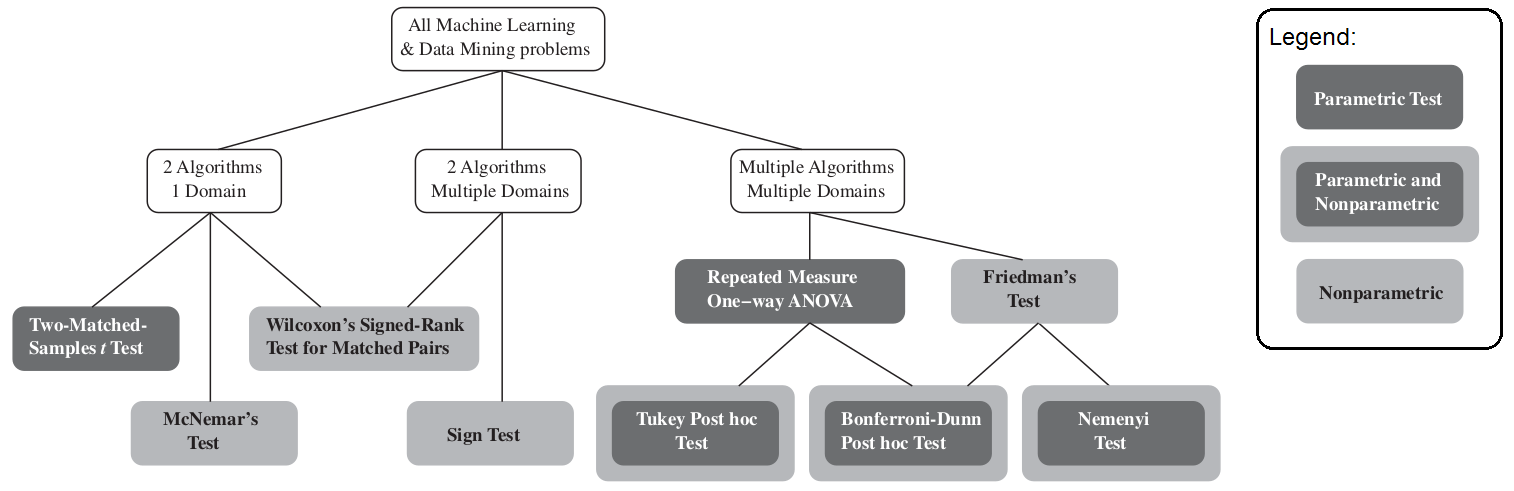
\includegraphics[width=\textwidth]{figure_man/tests_overview.png} \end{center}

\footnotesize
{\tiny{Source: \code{\url{https://marthawhite.github.io/mlcourse/lectures/2017/Lec20-MeasuringPerformance.pdf}}, p. 142.}\par}

\end{vbframe}

%\section{Compare 2 Models on a Single Domain}


% \begin{vbframe}{Weaknesses of parametric tests}
%
% \begin{itemize}
% \item \textbf{Commensurability:} One has to be able to compare the differences over the data
% sets, thus if the used performance measures have different properties for different
% tasks, this assumption might be violated.
% \item \textbf{Normal distribution:} Unless the number of data sets is greater then 30, asymptotically
% normal distributed differences can not be assumed. Due to the nature
% of the underlying results, even at more than 30 data sets, such tests might prove
% unreliable.
% \item \textbf{Outliers:} Extreme values might skew the statistics and thus decrease a tests
% power.
% \end{itemize}
%
% \end{vbframe}

\begin{vbframe}{McNemar test}
% https://slideplayer.com/slide/9574350/
\begin{itemize}
\item The \textbf{McNemar test} is a non-parametric test used on paired nominal data that does not make any distributional assumptions.
\item It can be applied to compare the performance of two \textbf{models} when the considered performance measure is based on an outer loss with a nominal or binary output, e.g., accuracy is based on a binary outer loss.
\item Both models are trained on a training set and evaluated on a test set. Based on the test set, a \textbf{contingency table} that compares the two models (model 1 and model 2) is calculated:
\end{itemize}

\begin{minipage}{0.34\textwidth}
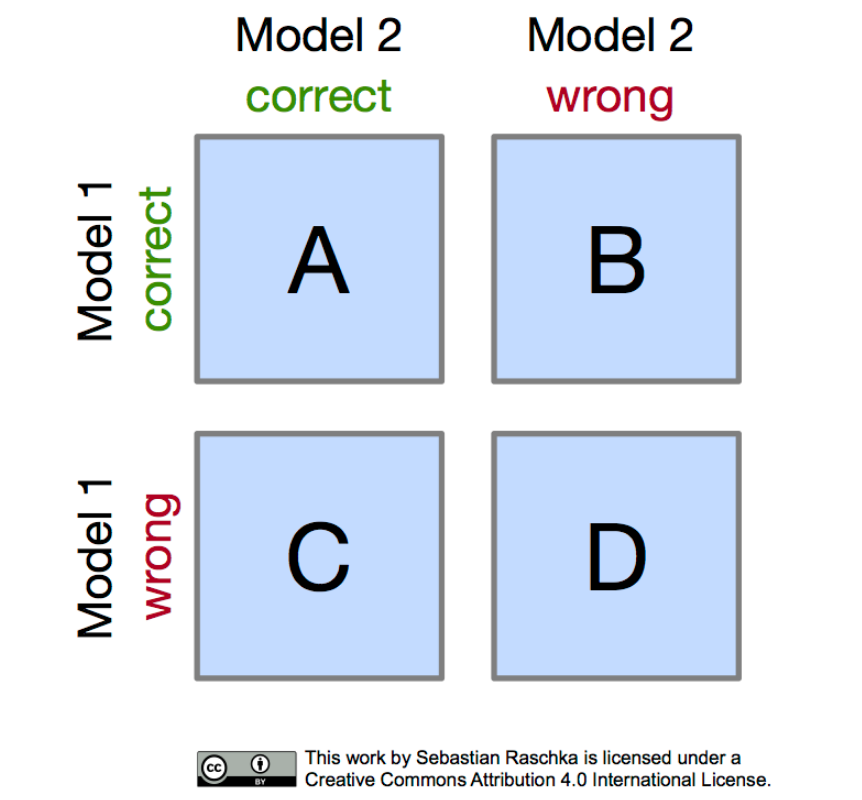
\includegraphics[width=\textwidth]{figure_man/mcnemar_1.png} \end{minipage}
\begin{minipage}{0.64\textwidth}
\begin{itemize}
\item A: $\#$ obs. correctly classified by both.
\item B: $\#$ obs. misclassified by model 2 but not by model 1.
\item C: $\#$ obs. misclassified by model 1 but not by model 2.
\item D: $\#$ obs. misclassified by both.
\end{itemize}
\end{minipage}
%
% \begin{minipage}[c]{0.4\linewidth}
%   \begin{center}
%   \renewcommand{\arraystretch}{1.5}
%   \begin{tabular}{cc|cc}
%       & & \multicolumn{2}{c}{$f_2$} \\
%       & & $0$ & $1$ \\
%       \hline
%       \multirow{2}{*}{ $f_1$} & $0$ & $c_{00}^{Mc}$ & $c_{01}^{Mc}$ \\
%       & $1$ & $c_{10}^{Mc}$ & $c_{11}^{Mc}$ \\
%   \end{tabular}
%   \end{center}
% \end{minipage} % no space if you would like to put them side by side
% \begin{minipage}[c]{0.59\linewidth}
% \vspace{0.15cm}
%   $c_{00}^{Mc} = \sum_{i=1}^{|S_{test}|} \left[ I(f_1(\mathbf{x_i}) \neq y_i) \wedge I(f_2(\mathbf{x_i}) \neq y_i) \right]$ \vspace{0.05cm}
%
%   $c_{01}^{Mc} = \sum_{i=1}^{|S_{test}|} \left[ I(f_1(\mathbf{x_i}) \neq y_i) \wedge I(f_2(\mathbf{x_i}) = y_i)\right]$ \vspace{0.05cm}
%
%   $c_{10}^{Mc} = \sum_{i=1}^{|S_{test}|} \left[ I(f_1(\mathbf{x_i}) = y_i) \wedge I(f_2(\mathbf{x_i}) \neq y_i)\right]$ \vspace{0.05cm}
%
%   $c_{11}^{Mc} = \sum_{i=1}^{|S_{test}|} \left[ I(f_1(\mathbf{x_i}) = y_i) \wedge I(f_2(\mathbf{x_i}) = y_i)\right]$
%
% \end{minipage}
% \vspace{0.5cm}
%
% Testing: $H_0$: $c_{01}^{Mc} = c_{01}^{Mc} = c_{null}^{Mc}$
%
% $$\chi^2_{Mc} =  \frac{(|c_{01}^{Mc} - c_{01}^{Mc}| - 1)^2}{c_{01}^{Mc} + c_{10}^{Mc}} \overset{approx}{\sim} \chi^2_{1,1-\alpha}$$
%
% If $c_{01}^{Mc} + c_{01}^{Mc} < 20$, approximation doesn't work, use binomial instead

\framebreak

\begin{minipage}[c]{0.625\linewidth}
Given such a contingency table, the accuracy of each model can be computed as follows:
\begin{itemize}
  \item Model 1: (A+B)/(A+B+C+D)
  \item Model 2: (A+C)/(A+B+C+D)
\end{itemize}

Even if the models have \textbf{equal} accuracy (indicating equal performance), cells B and C may differ because the models may misclassify different instances.
\end{minipage}
\begin{minipage}[c]{0.365\linewidth}
  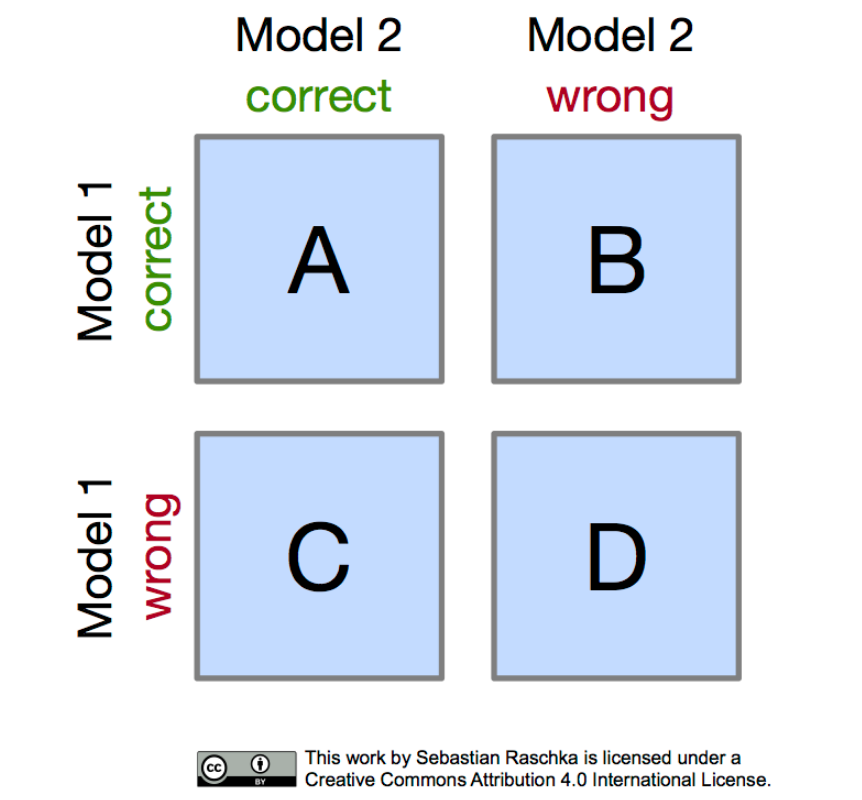
\includegraphics{figure_man/mcnemar_1.png}
\end{minipage}

\lz McNemar tests the following hypotheses:
\begin{itemize}
\item $H_0:$ Both models have the same performance (we expect B = C).
\item $H_1:$ Performances of the two models are not equal.
\end{itemize}
%\lz
The test statistic is computed by
$$\chi^2_{Mc} =  \tfrac{(|B-C| - 1)^2}{B + C} \sim \chi^2_{1}.$$

\textbf{Note}: The McNemar test should only be used if $B + C > 20$.

\framebreak

\textbf{Example}:

\begin{center}
  %\renewcommand{\arraystretch}{1.5}
%\hspace*{\fill}
  \begin{tabular}{cc|cc}
      & & \multicolumn{2}{c}{Random Forest} \\
      & & correct & wrong \\
      \hline
      \multirow{2}{*}{Tree} & correct & 30 & 5 \\
      & wrong & 17 & 42 \\
  \end{tabular}
\end{center}

Calculate the test statistic:

$$\chi^2_{Mc} =  \frac{(|5-17| - 1)^2}{5 + 17} = 5.5 > 3.841 = \chi^2_{1,0.95}.$$

We can reject $H_0$ at a significance level of 0.05, i.e., we reject the hypothesis that the tree and the random forest have the same performance.
% and assume that our tree and our random forest classify the data differently

% \framebreak
%
% \begin{itemize}
% \item McNemar test is a non-parametric test that compares the errors of two classifiers.
% \item classifiers have to be trained and tested on the same dataset.
% % \item $H_0$: the two classifiers have the same error rates, \\ $H_1$: the error rates differ
% \item Goodness-of-fit measure: Compares observed counts with expected distribution under $H_0$.
% \item Relies on contingency matrix and is very similar to $\chi^2$-Test.
% \item McNemar test considers if observations are classified correctly or not and does not provide any quantification of these measures.
% \item According Dietterich(1998), the McNemar test should only be used if $B + C > 20$.
% \end{itemize}
%
% \end{vbframe}

% \begin{vbframe}{T-test vs. McNemar Test}
%
% Apart from t-test being parametric and the McNemar test being non-parametric, two tests have other significant differences. Because of its nature, it is possible to construct intervals for t-test however it is not possible to work with intervals for McNemar test which only works with nominal performance measures. McNemar test takes into account that whether observations are classified correctly or not and it does not provide any quantification of these measures.
%
% \lz
%
% According to the Dietterich(1998), one can proceed with McNemar test when the number of disagreement between two classifiers $c_{01}^{Mc} + c_{01}^{Mc} $ is greater than 20.
%
\end{vbframe}


\begin{vbframe}{Two-matched-samples t-test}

A two-matched-samples t-test (i.e., a paired t-test) is the simplest hypothesis test if the aim is to compare two \textbf{models} on a single test set based on arbitrary performance measures.

However, it is a parametric test and distributional assumptions must be made (which are often problematic).

\lz The t-test relies on several assumptions:

\begin{itemize}
\item \textbf{(Pseudo-)normality}, usually met when sample size > 30.
\item \textbf{I.i.d. samples}, usually met if the loss of individual observations from a single test set is considered. % (this assumption is violated in case of resampling as ). %difficult as data is often limited (assumption is violated in the case of resampling).
\item \textbf{Equal variances of populations}, can be investigated by plots.
\end{itemize}

\framebreak

A paired t-test to compare two different models $\fh_1$ and $\fh_2$ w.r.t. a performance measure calculated on a test set of size $n_{\text{test}}$:

\begin{itemize}
\item $H_0$: $GE(\fh_{1}) = GE(\fh_{2})$ vs. $H_1$: $GE(\fh_{1}) \neq GE(\fh_{2})$
\item Test statistic $T = \sqrt{n_{\text{test}}} \frac{\bar{d}}{\sigma_{d}}$, with
%Teststatistic $t=\frac{d\left(\fh_A,\fh_B\right)}{\sqrt{\sigma_{A}^2 + \sigma_{B}^2}}$, with
\begin{itemize}
\item mean performance difference of both models
$\bar{d} = \GEh{\Dtest}(\fh_{1}) - \GEh{\Dtest}(\fh_{2})$, and
\item standard deviation of this mean difference
$$\sigma_{d} = \sqrt{\frac{1}{n_{\text{test}} - 1}\sum_{i=1}^{n_{\text{test}}} \left(d_i - \bar{d} \right)^2},$$
where $d_i = L(\yi, \fh_1 (\xi)) - L(\yi, \fh_2 (\xi))$ and $\bar{d} = \sum\limits_{i=1}^{n_{\text{test}}} d_i$.
%the variance of binomial distribution: \newline
\end{itemize}
\end{itemize}

\textbf{Note}: Here, $d_i$ is the difference of the outer loss of individual observations from the test set between the two models to be compared.
%\textbf{Issue}: $\GEh{n} \left(\fh_A\right)$ and $ \GEh{n} \left(\fh_B\right)$ are not independent as they are calculated on the same test set.

\begin{itemize}
\item We could also use a \textbf{$k$-fold CV paired t-test} to compare two \textbf{algorithms} (instead of two models) on a single dataset.
\item Instead of comparing the outer loss of individual observations we would then compare the individual generalization errors per CV fold (i.e., the generalization error of the $k$ prediction models induced by the learning algorithm in each CV fold).
%\item Instad of using the difference of the outer loss of individual observations
\item Although the test sets do not overlap, the performance differences are not independent across CV folds due to overlapping training sets (which violates the assumption of i.i.d. samples).
%However, the paired t-test is a parametric test and is not recommended in practice as the assumptions of the student's t-test are often violated.
%\item A probably better alternative is, therefore, the Friedman test.
\item To partly overcome the issue of overlapping training sets across folds, Dietterich\footnote{Dietterich (1998). Approximate statistical tests for comparing supervised classification learning algorithms.} suggests using 5 times 2-fold CV so that at least within each repetition neither the training nor the test sets overlap.
\end{itemize}
\end{vbframe}

%\section{Compare Multiple Models Multiple Domains}

\begin{vbframe}{Friedman test}
So far we have only compared 2 models / algorithms on one dataset. The \textbf{Friedman test} can be used to compare multiple classifiers on multiple datasets. The hypotheses to be tested are:
\begin{itemize}
\item $H_0:$ All algorithms are equivalent in their performance and hence their average ranks should be equal.
\item $H_1:$ The average rank for at least one algorithm is different.
\end{itemize}

\lz
Suppose we want to evaluate $m$ data sets and $k$ algorithms. A \textbf{Friedman test} is constructed as follows:

\begin{itemize}
  \item Separately rank each algorithm for each dataset from best-performing (rank 1) to worst-performing, using any performance measure of interest.
  \item If there is a $d$-way tie after rank $r$, assign a rank of $ \left[(r+1) + (r+2) + ... + (r+d)\right] /d $ to all tied classifiers.
  \item $R_{ij}$ is the rank of algorithm $j$ on data set $i$.
\end{itemize}

\end{vbframe}

\begin{vbframe}{Friedman test}
After obtaining the rank for each algorithm $j$ on different datasets $i$, calculate the following quantities:

\begin{itemize}
  \item The overall mean rank:
  $ \bar{R} = \frac{1}{mk} \sum_{i=1}^{m} \sum_{j=1}^{k} R_{ij}. $
  \item The total sum of squares:
  $ SS_{Total} = m \sum_{j=1}^{k} (\bar{R}_{.j} - \bar{R})^2 $, where $\bar{R}_{.j} =  \frac{1}{m} \sum_{i=1}^{m} R_{ij}$.
  \item The error sum of squares:
  $ SS_{Error} = \frac{1}{m(k-1)} \sum_{i=1}^{m} \sum_{j=1}^{k} (R_{ij} - \bar{R})^2. $
\end{itemize}

\lz

The Friedman test statistic is calculated as:

$${\chi_F}^2 = \frac{SS_{Total}}{SS_{Error}} \sim \chi_{k-1}^2 \text{ for large \textit{m} ($>15$) and \textit{k} ($>5$).}$$

In the case of smaller $m$ and $k$, the $\chi^2$ approximation is imprecise and a look-up of $\chi_F^2$ values that were approximated specifically for the Friedman test is suggested.
\end{vbframe}


\begin{vbframe}{Post-hoc tests}
A Friedman test checks if all algorithms are ranked equally or not. However, it does not provide information w.r.t. the best-performing algorithm.
To address this issue, post-hoc tests can be used.

\lz \textbf{Post-hoc Nemenyi test}:
\begin{itemize}
\item Compares all algorithms pairwise to find the best-performing algorithm after $H_0$ of the Friedman test was rejected.
\item For $m$ data sets and $k$ algorithms, $\frac{k(k-1)}{2}$ comparisons are made.
\item Calculates the average rank of algorithm $j$ on all $m$ data sets: $\bar{R}_{.j} =\frac{1}{m} \sum_{i=1}^m R_{ij}.$
\end{itemize}

\lz %The performance of two algorithms are significantly different when their average ranks differ by at least the significance level $q_{\alpha}$.
For any two algorithms $j_1$ and $j_2$, we compute the test statistic as:
$$q = \frac{\bar{R}_{.j_1} - \bar{R}_{.j_2}}{\sqrt{\frac{k(k+1)}{6m}}}.$$


\framebreak

\textbf{Post-hoc Bonferroni-Dunn test}:

\begin{itemize}
\item Compares all algorithms with a baseline (i.e., $k-1$ comparisons).
\item It is used after a Friedman test to find which algorithms differ from the baseline significantly.
\item It uses the Bonferroni correction to prevent randomly accepting one of the algorithms as significant due to multiple testing.
\end{itemize}
The test statistic is the same as before:
$$q = \frac{\bar{R}_{.j_1} - \bar{R}_{.j_{baseline}}}{\sqrt{\frac{k(k+1)}{6m}}}.$$

The performances of $j_1$ and $j_2$ differ significantly if $|q| > q_{\alpha}$, where the critical value $q_{\alpha}$ is obtained from a table of the studentized range statistic, scaled through division by $\sqrt{2}$.
%Another difference between Bonferroni-Dunn Test with Nemenyi test is that total number of comparisons are 1/k of Nemenyi test.
\end{vbframe}

% \begin{vbframe}{ROC Analysis}
%
% Any binary classifier $\hx$ can be characterized by its
% \begin{itemize}
%   \item true positive rate: $\text{TPR} = \cfrac{\text{\#TP}}{\text{\#TP} + \text{\#FN}}$ (Sensitivity, Recall)
%   \item false positive rate: $\text{FPR} = 1-\text{specificity} = \cfrac{\text{\#FP}}{\text{\#FP} + \text{\#TN}}$
% \end{itemize}
% \lz
%
% For a given scoring classifier $\fx$, define the associated binary classifier $h(x, \theta) = \I(f(x) \geq \theta)$ with decision threshold $\theta$.
% \lz
%
% The \textbf{R}eceiver \textbf{O}perating \textbf{C}haracteristic (ROC) curve of a scoring classifier is created by plotting \textit{tpr} vs. \textit{fpr} for all possible decision thresholds $\theta$.\\
% (Any given binary classifier occupies a single point (tpr, fpr)  in \enquote{ROC-Space}.)
%
% \framebreak
%
% ROC curves are insensitive to the class distribution in the sense that they are not affected by changes in the ratio $\np/\nn$:
%
% \begin{table}[]
% \centering
% \begin{tabular}{|l|c|c|}
%                 \hline
%    $\np/\nn = 1$            & True Positive & True Negative \\ \hline
% Pred. Positive & 40            & 25            \\ \hline
% Pred. Negative & 10            & 25           \\ \hline
% \end{tabular}
% \end{table}
% \begin{table}[]
% \centering
% \begin{tabular}{|l|c|c|}
%                 \hline
%      $\np/\nn = 2$        & True Positive & True Negative \\ \hline
% Pred. Positive & 80            & 25            \\ \hline
% Pred. Negative & 20            & 25           \\ \hline
% \end{tabular}
% \end{table}
%
% True positive rates ($\text{TPR} = 0.8$) and false positive rates ($\text{FPR} = 0.5$) do not change.


% \begin{itemize}
%   \item Note that the class distribution is
% the relationship of the left column to the right column.
%   \item Any performance metric that uses values from both
% columns will be inherently sensitive to class skews (such as accuracy, precision, F measure)
%   \item ROC curves are based upon tpr and fpr.
%   \item Each measure uses only values in their respective columns.
%   \item Changing the class distribution will therefore not change the ROC curve.
% \end{itemize}

%\end{vbframe}

\endlecture
\end{document}
